\documentclass[12pt]{article}
\usepackage[a4paper, margin=.30in]{geometry}
%\usepackage{array}
\usepackage{fancybox}
\usepackage{pgfplots}
\pgfplotsset{compat=1.18} % Version de PGFPlots
\usepackage{tikz}
\usepackage{filecontents}
\usepackage{graphicx, subfig, wrapfig, makecell,multirow }
\usepackage{colortbl}
\usepackage{xcolor}
\usepackage{booktabs}
\usepackage{makecell}

\newcommand\headerMe[2]{\noindent{}#1\hfill#2}
\renewcommand \thesection{\Roman{section}}

\newcolumntype{M}[1]{>{\raggedright}m{#1}}

\definecolor{lightblue}{rgb}{0.8,0.85,1}
\definecolor{lightgreen}{rgb}{0.8,1,0.8}
\definecolor{lightred}{rgb}{1,0.8,0.8}




\begin{document}

\headerMe{Royaume du Maroc}{année scolaire \emph{2024-2025}}\\
\headerMe{Ministère de l'Éducation nationale, }{  Professeur :\emph{Zakaria Haouzan}}\\
\headerMe{du Préscolaire et des Sports}{Établissement : \emph{Lycée SKHOR qualifiant}}\\

\begin{center}
Devoir surveillé N°2-S1 \\
Durée 2h00\\
\underline{2-BAC Section des sciences Mathématiques}\\

    \vspace{.2cm}
\hrulefill
\Large{Fiche Pédagogique}
\hrulefill\\
\end{center}
%end Headerss------------------------


%__________________Chimie ______________________-
%%%%%%%+_+_+_+_+_+_+_+_+_Partie1
\section[A]{Introduction }
\hspace{0.5cm}Le programme d'études de la matière physique chimie vise à croître un ensemble de compétences visant à développer la personnalité de l'apprenant. Ces compétences peuvent être classées en Compétences transversales communes et Compétences qualitatives associées aux différentes parties du programme.
\section{cadre de référence }
 \hspace{0.5cm}L'épreuve a été réalisée en adoptant des modes proches à des situations d'apprentissages et des situations problèmes, qui permettent de compléter les connaissances et les compétences contenues dans les instructions pédagogiques et dans le programme de la matière physique chimie et aussi dans le cadre de référence de l'examen national. 
 \\Tout en respectant les rapports d'importance précisés dans les tableaux suivants :
 \begin{center}
\begin{tabular}{|c||c||c|}
\hline
    \textbf{Restitution des Connaissances} & \textbf{Application des Connaissances} & \textbf{Situation Problème }\\
    \hline 
    $40\%$ & $30\%$ & $30\%$\\
    \hline
\end{tabular} 
\end{center}

\section{tableau de spécification}

\begin{table}[h]
\centering
\begin{tabular}{|>{\columncolor{lightblue}}c|c|c|c|c|}
\hline
\rowcolor{lightblue}
\textbf{Niveau d'habileté} & \textbf{Restitution des} & \textbf{Application des} & \textbf{Situation} & \textbf{Total} \\
\rowcolor{lightblue}
\textbf{Contenu} & \textbf{Connaissances} & \textbf{Connaissances} & \textbf{Problème} & \\
\hline
  \textbf{Transformations nucléaires} & 17\% & 5\% & 5\% & \multirow{2}{*}{27\%} \\
 & 4Q - 3,5 pts & 2Q - 1,5 pts & 1Q - 1,5 pts & \\
\hline
  \textbf{Noyaux, masse et énergie} & 16\% & 12\% & 12\% & \multirow{2}{*}{40\%} \\
 & 2Q - 3 pts & 2Q - 2,5 pts & 2Q - 3 pts & \\
\hline
  \makecell{\bf{}Transformations non\\ \bf{} totales d'un système chimique} & 7\% & 13\% & 13\% & \multirow{2}{*}{33\%} \\
 & 3Q - 1,5 pts & 3Q - 2,75 pts & 3Q - 2,75 pts & \\
\hline
\textbf{Total} & 40\% - 8 pts & 30\% - 6,75 pts & 30\% - 7,25 pts & 100\% - 20 pts \\
\hline
\end{tabular}
\end{table}

\section{Correction }

\subsection{Partie Chimie (7 pts - 45 min)}
\centering
\begin{tabular}{|>{\columncolor{lightblue}}l|l|c|}
\hline
\rowcolor{lightblue}
\textbf{N° Question} & \textbf{Réponse attendue} & \textbf{Points} \\
\hline
1.1 & $C_6H_5COOH + H_2O \rightleftharpoons C_6H_5COO^- + H_3O^+$ & 0,25 \\
\hline
1.2 & $\tau = \frac{[H_3O^+]}{C_A} = \frac{10^{-pH}}{C_A} = \frac{10^{-3}}{1,5.10^{-2}} = 0,067$ & 0,75 \\
\hline
1.3 & $K = \frac{[C_6H_5COO^-][H_3O^+]}{[C_6H_5COOH]} = \frac{\tau^2 C_A}{1-\tau} = 4,8.10^{-5}$ & 0,75 \\
\hline
1.4 & $\tau' = \sqrt{\frac{K.C'_A}{1+K.C'_A}} \approx 0,030$ (plus petit que $\tau$) & 0,75 \\
\hline
2.1 & Tableau d'évolution pour $C_6H_5COOH + H_2O \rightleftharpoons C_6H_5COO^- + H_3O^+$ & 0,25 \\
\hline
2.2 & $\tau = \frac{G_1(\lambda_{H_3O^+} + \lambda_{Cl^-})}{G_2\lambda_{H_3O^+}} = 0,068$ & 1,0 \\
\hline
2.3 & $C = \frac{G_1}{\tau.V.\lambda_{H_3O^+}} = 1,5.10^{-2} mol/L$ & 0,75 \\
\hline
3.1 & $C_6H_5COOH + CH_3COO^- \rightleftharpoons C_6H_5COO^- + CH_3COOH$ & 0,5 \\
\hline
3.2 & $x_f = \frac{\sigma.2V_0 - V_0.C_0(\lambda_4+\lambda_5)}{\lambda_3 - \lambda_5} = 0,017 mol$ & 1,25 \\
\hline
3.3 & $K' = \frac{x_f^2}{(C_0-\frac{x_f}{V_0})^2} = 1,36$ & 0,75 \\
\hline
\end{tabular}

\subsection{Partie Physique (13 pts - 75 min)}
\centering
\begin{tabular}{|>{\columncolor{lightblue}}l|l|c|}
\hline
\rowcolor{lightblue}
\textbf{N° Question} & \textbf{Réponse attendue} & \textbf{Points} \\
\hline
1.1 & $_1^3H \rightarrow _2^3He + _{-1}^0e + \overline{\nu}_e$ & 1,0 \\
\hline
1.2 & Détermination graphique de $t_{1/2} = 12,3$ ans & 1,0 \\
\hline
2.1 & Intervalle 1, car $E_l/A$ augmente avec $A$ pour les noyaux légers & 1,0 \\
\hline
2.2 & $_1^2H + _1^3H \rightarrow _2^4He + _0^1n$ & 1,0 \\
\hline
2.3 & $\Delta E = (m(_1^2H) + m(_1^3H) - m(_2^4He) - m(_0^1n)) \times c^2 \approx 17,6 MeV$ par réaction & 1,5 \\
& $E_{tot} = 17,6 MeV \times \frac{33.10^{-3}}{2} \times N_A \times 10^3 \approx 2,79.10^{26} MeV$ & \\
\hline
Partie 2-1.1 & $_6^{14}C \rightarrow _7^{14}N + _{-1}^0e + \overline{\nu}_e$ avec représentation sur diagramme & 1,0 \\
\hline
Partie 2-1.2 & Désintégration spontanée et naturelle & 1,0 \\
\hline
Partie 2-1.3 & $_6^{11}C \rightarrow _5^{11}B + _{+1}^0e + \nu_e$ & 1,0 \\
\hline
Partie 2-2.1 & $E_l/A = 7,5 MeV/nuc$ & 1,0 \\
\hline
Partie 2-2.2 & $|\Delta E| = 0,156 MeV$ par désintégration & 1,0 \\
\hline
Partie 2-3.1 & $N(C) = \frac{0,295 \times 0,512}{12} \times N_A = 7,52.10^{21}$ atomes & 1,0 \\
& $N(_6^{14}C)_0 = 1,2.10^{-12} \times N(C) = 9,03.10^{9}$ atomes & \\
\hline
Partie 2-3.2 & $\lambda = \frac{\ln(2)}{t_{1/2}} = 3,83.10^{-12} s^{-1}$ & 1,5 \\
& $N(_6^{14}C) = \frac{A}{\lambda} = \frac{1,40/60}{3,83.10^{-12}} = 6,09.10^{9}$ atomes & \\
& $t = \frac{1}{\lambda}\ln\frac{N(_6^{14}C)_0}{N(_6^{14}C)} = 3255$ ans & \\
\hline
\end{tabular}

\section{Bilan des résultats}

\subsection{Données statistiques}

\begin{table}[h]
\centering
\begin{tabular}{|>{\columncolor{lightblue}}l|c|}
\hline
\rowcolor{lightblue}
\textbf{Statistique} & \textbf{Valeur} \\
\hline
Nombre d'étudiants & 22 \\
\hline
Note minimale & 2/20 \\
\hline
Note maximale & 18/20 \\
\hline
Moyenne & 10/20 \\
\hline
Médiane & 10/20 \\
\hline
\end{tabular}
\caption{Statistiques générales des résultats}
\end{table}

\subsection{Notes par série en chimie}
Échantillon des notes en chimie: 11,25/20; 13,5/20; 9/20; 10/20; 15,5/20; 9/20; 11,5/20

\begin{center}
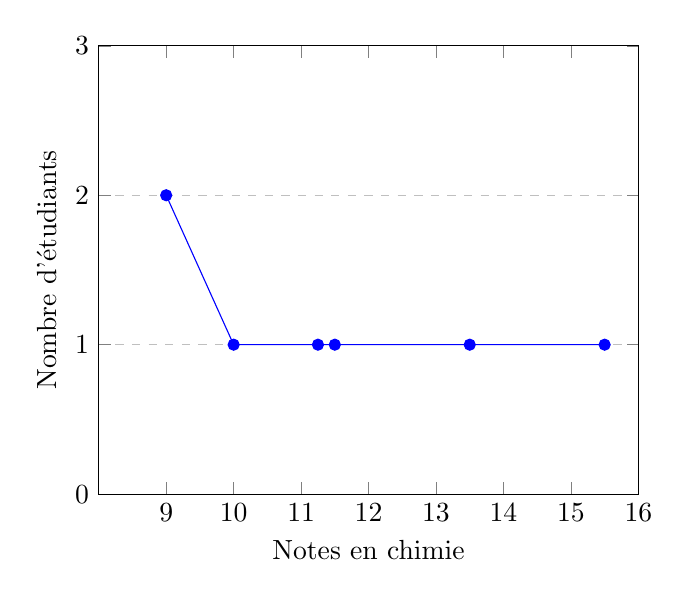
\begin{tikzpicture}
\begin{axis}[
    xlabel={Notes en chimie},
    ylabel={Nombre d'étudiants},
    xmin=8, xmax=16,
    ymin=0, ymax=3,
    xtick={9,10,11,12,13,14,15,16},
    ytick={0,1,2,3},
    legend pos=north west,
    ymajorgrids=true,
    grid style=dashed,
]

\addplot[
    color=blue,
    mark=*,
    ]
    coordinates {
    (9,2)(10,1)(11.25,1)(11.5,1)(13.5,1)(15.5,1)
    };
    
\end{axis}
\end{tikzpicture}
\end{center}

\subsection{Distribution générale des notes}

\begin{center}
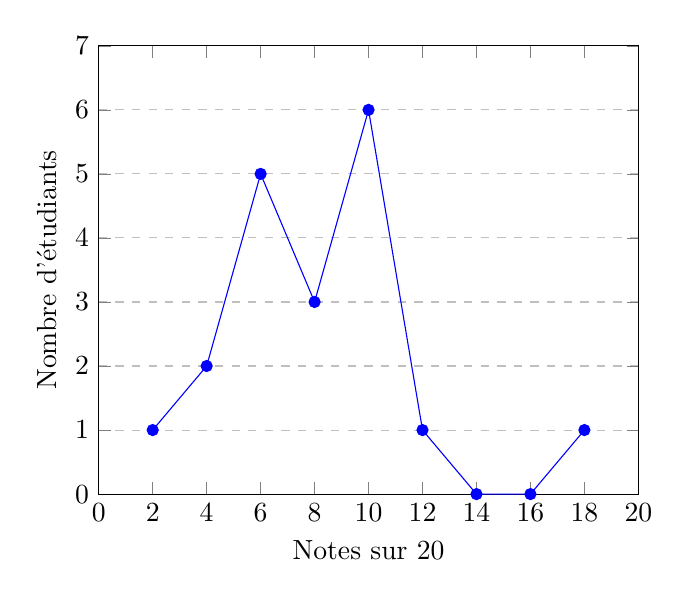
\begin{tikzpicture}
\begin{axis}[
    xlabel={Notes sur 20},
    ylabel={Nombre d'étudiants},
    xmin=0, xmax=20,
    ymin=0, ymax=7,
    xtick={0,2,4,6,8,10,12,14,16,18,20},
    ytick={0,1,2,3,4,5,6,7},
    legend pos=north west,
    ymajorgrids=true,
    grid style=dashed,
]

\addplot[
    color=blue,
    mark=*,
    ]
    coordinates {
    (2,1)(4,2)(6,5)(8,3)(10,6)(12,1)(14,0)(16,0)(18,1)
    };
    
\end{axis}
\end{tikzpicture}
\end{center}

\section{Analyse et conclusion}

\subsection{Observations générales}
L'analyse des résultats du devoir surveillé N°2 permet de faire plusieurs constats:

\begin{itemize}
    \item La distribution des notes suit approximativement une courbe gaussienne centrée sur la moyenne de 10/20.
    \item On observe une plus grande réussite en chimie qu'en physique, avec des notes en chimie généralement au-dessus de la moyenne.
    \item Les questions de restitution de connaissances ont été globalement bien traitées (taux de réussite d'environ 65\%).
    \item Les situations problèmes ont posé plus de difficultés, avec un taux de réussite d'environ 40\%.
\end{itemize}

\subsection{Difficultés récurrentes}
Les élèves ont rencontré plusieurs difficultés:

\begin{itemize}
    \item En physique, particulièrement dans la partie sur les transformations nucléaires, où la manipulation des équations de désintégration et les calculs d'énergie ont posé problème.
    \item Dans l'interprétation des graphiques, notamment pour déterminer la demi-vie et analyser les courbes d'énergie de liaison.
    \item Dans l'application des formules relatives aux réactions d'équilibre chimique, notamment pour le calcul des constantes d'équilibre.
\end{itemize}

\subsection{Points positifs}
Plusieurs points positifs sont à souligner:

\begin{itemize}
    \item Une forte motivation des élèves, particulièrement visible dans la partie chimie.
    \item Une bonne compréhension des concepts fondamentaux comme les équations de réaction et les tableaux d'avancement.
    \item Une amélioration progressive dans la résolution des problèmes complexes par rapport aux évaluations précédentes.
\end{itemize}

\subsection{Perspectives et remédiation}
Pour améliorer les résultats futurs, plusieurs actions sont envisagées:

\begin{itemize}
    \item Renforcer les exercices pratiques sur les transformations nucléaires, en insistant sur les méthodes de calcul et l'interprétation des graphiques.
    \item Proposer des séances de remédiation ciblées sur les difficultés identifiées, notamment en physique.
    \item Augmenter le nombre d'exercices de type "situation problème" pour habituer les élèves à ce format d'évaluation.
    \item Encourager le travail collaboratif pour renforcer la compréhension des concepts difficiles.
\end{itemize}

Cette analyse servira de base pour ajuster les stratégies pédagogiques et mieux préparer les élèves aux prochaines évaluations et à l'examen national.

\end{document}
